\documentclass[border=0pt]{standalone}
\usepackage{amsmath}

%%font
\usepackage{euler}
\usepackage[OT1]{eulervm}
\renewcommand{\rmdefault}{pplx}

\usepackage{tikz}
\tikzset{every node/.style={draw, circle, inner sep=3pt}}
\usetikzlibrary{arrows}
\definecolor{TortugaColor}{rgb}{0.1,0.4,0.3}

%% Layers setup
\pgfdeclarelayer{background}
\pgfdeclarelayer{alpha}
\pgfdeclarelayer{beta}
\pgfsetlayers{background,alpha,main,beta}

\parindent=0pt

\begin{document}
%% 1/3 Haitian
%% 16:9
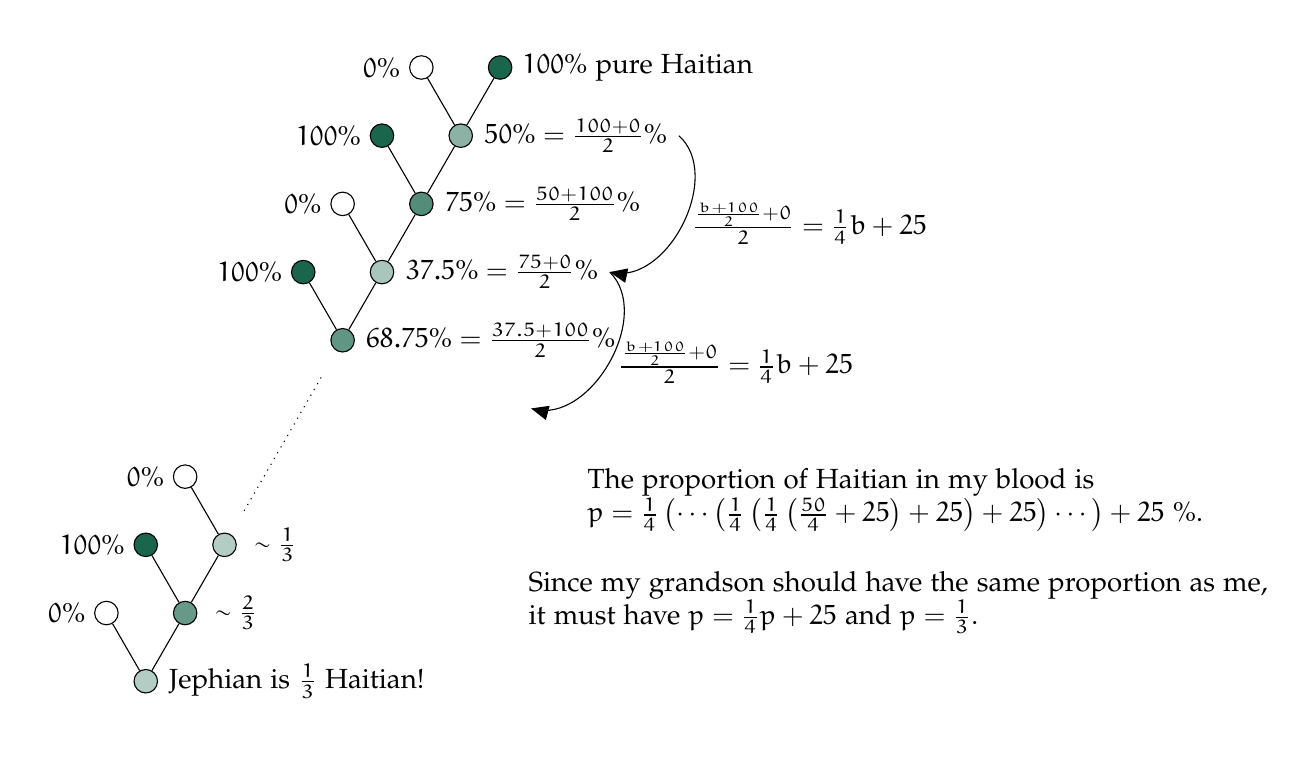
\begin{tikzpicture}
\coordinate (Jamaica) at (-8,-4);
\coordinate (Dominican) at (8,-4);
\coordinate (Cuba) at (-8,5);
\coordinate (TurksCaicos) at (8,5);
\coordinate (Tortuga) at (0,0);
\clip (Jamaica) rectangle (TurksCaicos);

%%Help Lines
\begin{pgfonlayer}{beta}
%\draw [step=1, black!50, thin] (Jamaica) grid (TurksCaicos);
%\draw (0,0) circle [radius=0.5cm];
\end{pgfonlayer}

\begin{pgfonlayer}{main}

\begin{scope}[shift={(-6.5,-3.3)},rotate=60]
\node[label={right:Jephian is $\frac{1}{3}$ Haitian!}, fill=TortugaColor!33.33] (0) at (0,0) {};
\node[label={right:$\sim \frac{2}{3}$}, fill=TortugaColor!66.66] (1) at (1,0) {};
\node[label={right:$\sim \frac{1}{3}$}, fill=TortugaColor!33.33] (2) at (2,0) {};
\node[label={right:$68.75\%=\frac{37.5+100}{2}\%$}, fill=TortugaColor!68.75] (3) at (5,0) {};
\node[label={[name=l4]right:$37.5\%=\frac{75+0}{2}\%$}, fill=TortugaColor!37.5] (4) at (6,0) {};
\node[label={right:$75\%=\frac{50+100}{2}\%$}, fill=TortugaColor!75] (5) at (7,0) {};
\node[label={[name=l6]right:$50\%=\frac{100+0}{2}\%$}, fill=TortugaColor!50] (6) at (8,0) {};
\node[label={right:$100\%$ pure Haitian}, fill=TortugaColor] (7) at (9,0) {};
\draw[dotted] (2.5,0) -- (4.5,0);
\end{scope}
\draw (0) -- (1) -- (2);
\draw (3) -- (4) -- (5) -- (6) -- (7);
\draw[-triangle 45] (l6.east) [bend left=75]to node[midway,right,draw=none,rectangle] {$\frac{\frac{b+100}{2}+0}{2}=\frac{1}{4}b+25$} (l4.east);
\draw[-triangle 45] (l4.east) [bend left=75]to node[midway,right,draw=none,rectangle] {$\frac{\frac{b+100}{2}+0}{2}=\frac{1}{4}b+25$} ++(-120:2);


\begin{scope}[every label/.style={shift={(120:-1)},rectangle,draw=none}, every node/.append style={shift={(120:1)}}]
\node[label={left:$0\%$},fill=TortugaColor!0] (p0) at (0) {};
\node[label={left:$100\%$},fill=TortugaColor!100] (p1) at (1) {};
\node[label={left:$0\%$},fill=TortugaColor!0] (p2) at (2) {};
\node[label={left:$100\%$},fill=TortugaColor!100] (p3) at (3) {};
\node[label={left:$0\%$},fill=TortugaColor!0]  (p4) at (4) {};
\node[label={left:$100\%$},fill=TortugaColor!100]    (p5) at (5) {};
\node[label={left:$0\%$},fill=TortugaColor!0]    (p6) at (6) {};
\end{scope}
\foreach \i in {0,...,6}{
\draw (p\i)--(\i);
}

\node[right,rectangle,draw=none,align=left] at (-1,-1) {
The proportion of Haitian in my blood is \\ 
$p=\frac{1}{4}\left(\cdots\left(\frac{1}{4}\left(\frac{1}{4}\left(\frac{50}{4}+25\right)+25\right)+25\right)\cdots\right)+25~\%$.};

\node[shift={(-120:1.5)},right,rectangle,draw=none,align=left] at (-1,-1) {
Since my grandson should have the same proportion as me,\\
it must have $p=\frac{1}{4}p+25$ and $p=\frac{1}{3}$.};
\end{pgfonlayer}



\end{tikzpicture}
\end{document}